%versi 2 (8-10-2016)
\chapter{Landasan Teori}
\label{chap:teori}

\section{KIRI Website }
\label{sec:KIRI} 
KIRI adalah aplikasi navigasi angkutan umum berbasis web yang melayani Bandung dan kota-kota lain di Indonesia.\cite{pascal:17:KIRI}.
Pada awal pembuatannya KIRI dibuat untuk tujuan komersial. Namun karena dinilai kurang sukses project KIRI sekarang menjadi open source project yang dapat di akses di url: \url{https://projectkiri.id/}. Aplikasi KIRI memiliki beberapa fitur sebagai berikut:
\begin{itemize}
    \item Pemilihan rute tercepat menggunakan angkutan kota.
    \item Menampilkan tempat pergantian angkutan kota.
    \item Memiliki fitur multi bahasa.
    \item Memiliki fitur pemilihan lokasi.
    \item Dapat menampilkan beberapa pilihan rute.
    \item Dapat menampilkan instruksi lengkap  mencapai tujuan.
\end{itemize}

\begin{figure}[H]
    \centering
    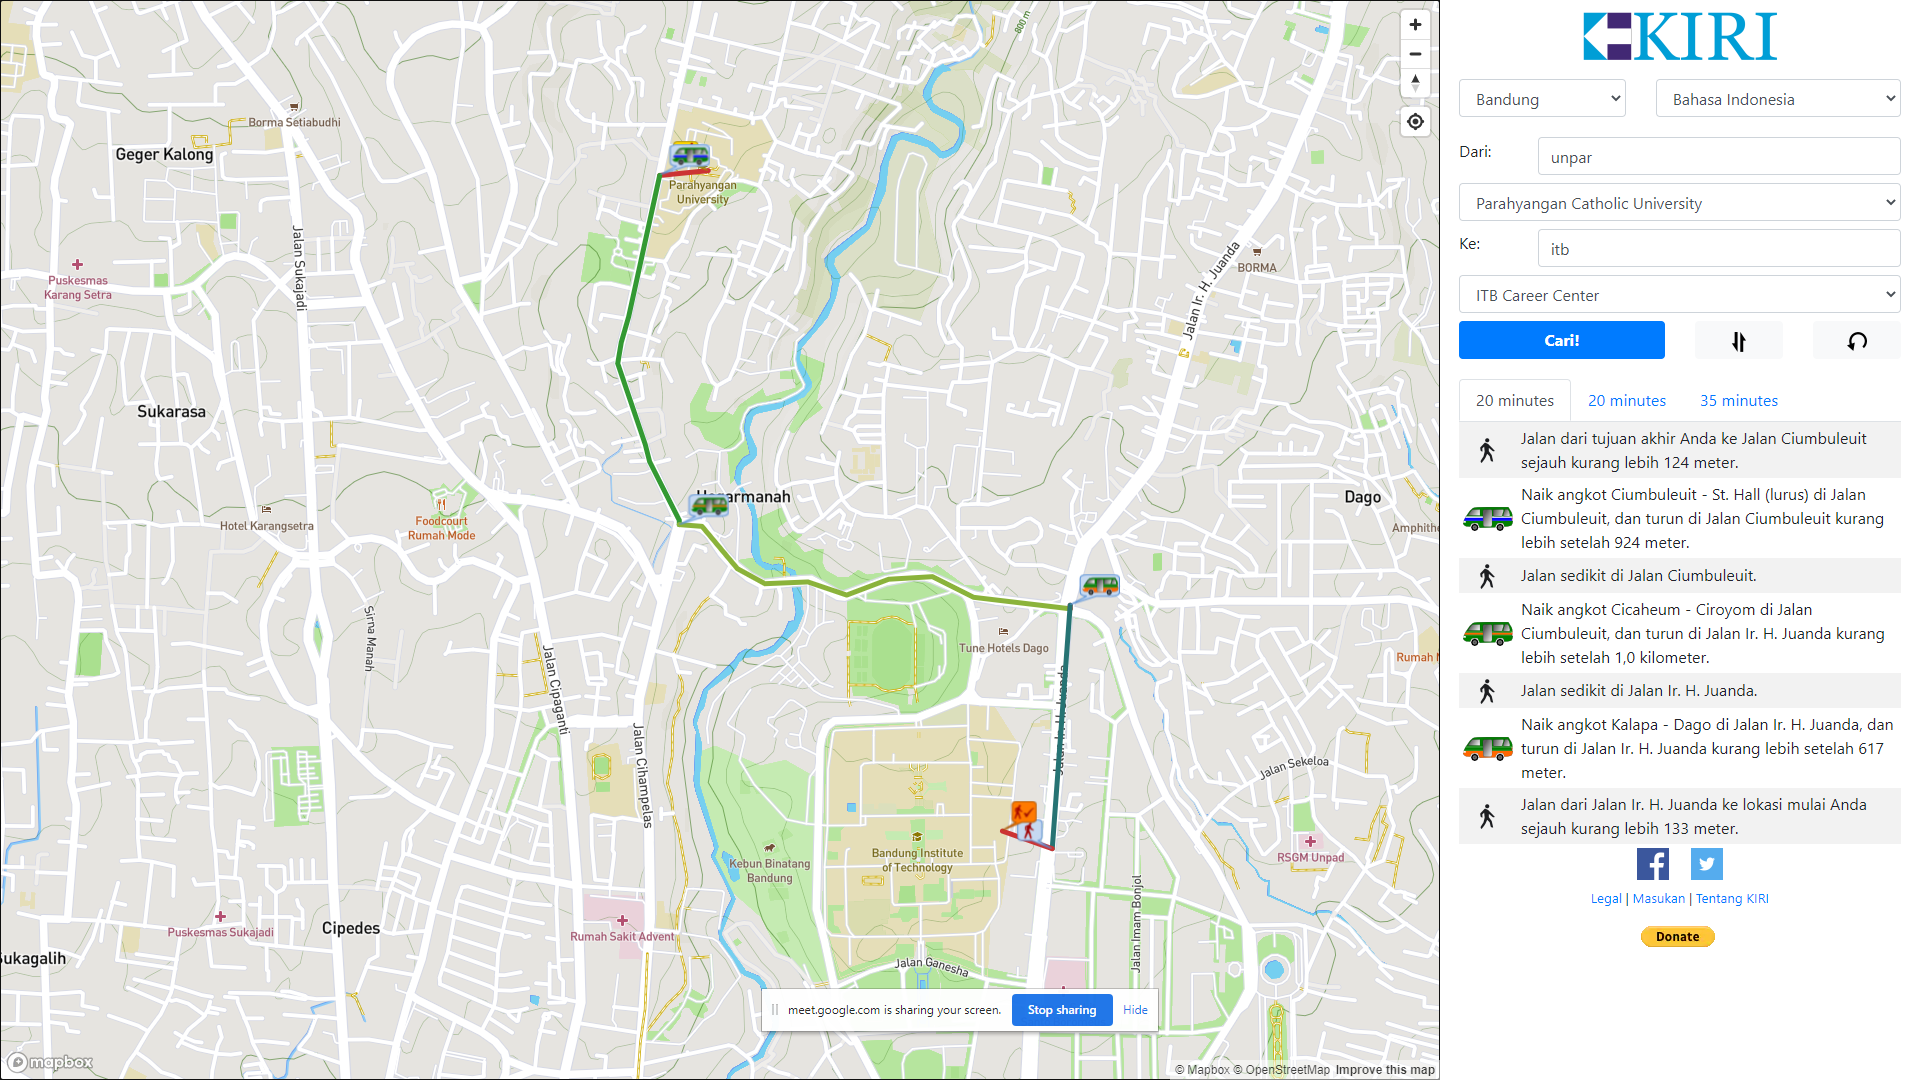
\includegraphics[scale=0.3]{Gambar/kiri-example-1}
    \caption{Tampilan utama website KIRI}
    \label{fig:my_label}
\end{figure}




\section{JSON}
\label{subsec:json}
JSON (\textit{JavaScript Object Notation}) adalah notasi berbasis teks,
   format pertukaran data bahasa-independen. berasal dari
   Standar Bahasa Pemrograman ECMAScript \footnote{https:\slash \slash tools.ietf.org/html/rfc7159}. JSON merupakan format teks yang tidak bergantung pada bahasa pemprograman apapun karena menggunakan gaya bahasa yang umum digunakan oleh bahasa pemrograman C termasuk C, C++, C\#, Java, JavaScript, Perl, Python, dan lain-lain. Oleh karena sifat-sifat tersebut, menjadikan JSON ideal sebagai bahasa pertukaran-data. JSON memiliki enam tipe data, yaitu \textit{string}, angka, \textit{null}, \textit{array} (ditandai dengan tanda kurung siku ($\left [ \right ]$)), \textit{object} (ditandai dengan tanda kurung kurawal (\{\})), dan \textit{boolean} (\textit{true} dan \textit{false}). Struktur utama JSON terdiri dari pasangan nama atau nilai yang dipisahkan dengan tanda titik dua (:). Contoh struktur JSON mengenai tipe dan jenis atribut dapat dilihat pada Listing~ \ref{listing:JSON}.

\begin{lstlisting}[caption=Contoh Struktur JSON, label=listing:JSON]
 {
 "timestamp":"2014-1-2:0:11",
 "start":"-6.8972513,107.6385574",
 "finish":"-6.91358,107.62718"
 }
\end{lstlisting}

\section{CSV}
\label{subsec:csv}
CSV (\textit{Comma Separated Values}) adalah suatu format data dalam basis data di mana setiap nilai atribut dipisahkan dengan tanda koma (,) dan setiap baris data ditandai dengan baris baru.\footnote{https:\slash \slash tools.ietf.org/html/rfc4180} CSV digunakan untuk bertukar data dan mengonversi data dari sebuah program \textit{spreadsheet} ke program \textit{spreadsheet} lainnya. Contoh CSV dapat dilihat pada Listing~\ref{listing:CSV}.

\begin{lstlisting}[caption=Contoh CSV, label=listing:CSV]
    logId,APIKey,Timestamp (UTC),Action,AdditionalData
    113909,E5D9904F0A8B4F99,2/1/2014 0:07,PAGELOAD,/5.10.83.30/
    113910,E5D9904F0A8B4F99,2/1/2014 0:07,PAGELOAD,/5.10.83.49/
\end{lstlisting}
	
\section{Google Maps Javascript API}
\label{sec:googlemaps}
Google Maps adalah layanan pemetaan web yang dikembangkan oleh Google. Menawarkan citra satelit, foto udara, dan peta jalan yang interaktif, kondisi lalu lintas secara \textit{real time} \cite{mehta:19:gmaps}.
Google Maps dalam service nya telah menyediakan \textit{API (pplication programming interface)} yang dapat di gunakan untuk public.
aplication programming interface adalah \textit{computer interface} yang mengatur komunikasi antar perangkat lunak \cite{libby:20:api}.
Google Maps telah menyediakan beberapa teknik pemetaan data yaitu :
 \begin{itemize}
     \item \textit{Heat Map}
     \item \textit{Marker Clustering}

 \end{itemize}
 \subsection{\textit{Heat Map}}
 \label{subsec:heat map}
 \textit{Heat Map} merupakan salah satu teknologi visualisasi yang merepresentasikan data kedalam gradien warna.\footnote{https://developers.google.com/maps/documentation/javascript/heatmaplayer} warna. Warna yang biasa digunakan adalah merah, kuning, hijau, dan biru.Warna-warna tersebut mencerminkan banyak data dari yang terbanyak sampai paling sedikit dengan urutan merah ke kuning ke hijau ke biru.Heatmap bisa digunakan untuk visualisasi data yang berbentuk 2-D dan 3-D.
 \textit{Heatmap 2-D} digunakan untuk membuat grafik berbentuk tabel untuk menyajikan data dalam baris dan kolom secara simultan. Selain berbentuk grafik \textit{heatmap 2-D} juga digunakan untuk membuat simulasi persebaran data. \textit{Heatmap 3D} digunakan untuk membuat grafik 3-D. \textit{Heatmap 3-D} juga bisa digunakan untuk membuat simulasi tekanan gelombang dan bisa juga digunakan untuk membuat \textit{surface plot}.
 \textit{Heatmap} juga bisa digunakan untuk mengelompokkan data berdasarkan jumlah atau berdasarkan kerapatan dari kumpulan data. Kelebihan dari \textit{heatmap} adalah \textit{heatmap} dapat mengelompokkan data secara otomatis dari jumlah terbanyak sampai jumlah paling sedikit.  \footnote{https://www.hotjar.com/heatmaps/}
 
 \begin{figure}[H]
    \centering
    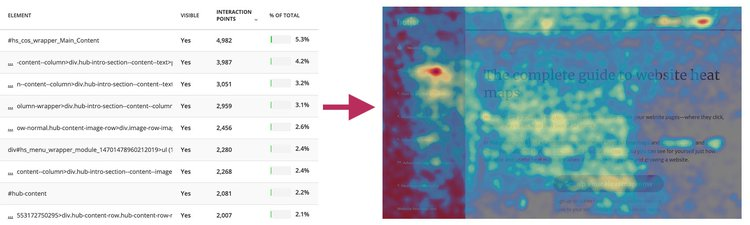
\includegraphics[scale=0.5]{Gambar/Heatmap-data-visualization.width-750.jpg}
    \caption{Contoh \textit{Marker Clustering}}
    \label{fig:my_label}
\end{figure}


 
 \subsection{\textit{Marker Clustering}}
 \label{subsec:heat map}
 \textit{Marker Clustering } merupakan teknik visualisasi  dimana akan melakukan \textit{clustering} pada \textit{pin} pada peta sehingga dapat mempermudah pengguna untuk melihat \textit{pin} pada tingkat \textit{zoom} tertentu. 
 \begin{figure}[H]
    \centering
    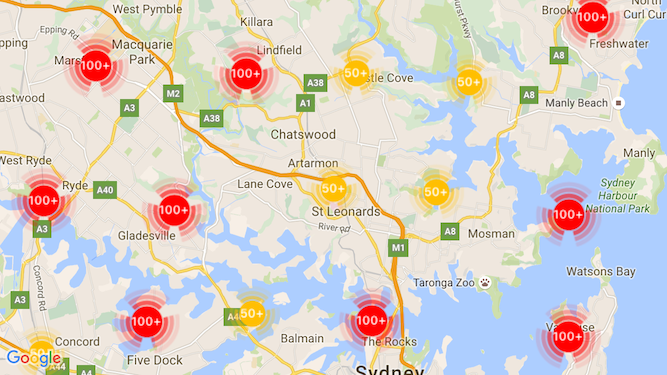
\includegraphics[scale=0.5]{Gambar/markerclustering.png}
    \caption{Contoh \textit{Marker Clustering}}
    \label{fig:my_label}
\end{figure}

\textit{Marker Clustering} memiliki beberapa keuntungan memungkinkan peta dengan ribuan \textit{pin} dimuat dengan sangat cepat.Kelebihan menggunakan \textit{Marker Clustering} mampu untuk mengelompokan ribuan \textit{pin} dalam peta sehingga dapat memberikan hasil yang lebih \textit{readable} dan mudah di pahami oleh pengguna.\footnote{https://developers.google.com/maps/documentation/javascript/marker-clustering}